\documentclass[11pt]{article}
\usepackage{amssymb}
\usepackage{amsmath}
\usepackage{color}
\usepackage{tikz}
\usetikzlibrary{shapes,backgrounds}
\usetikzlibrary{arrows.meta, positioning, quotes}

\begin{document}

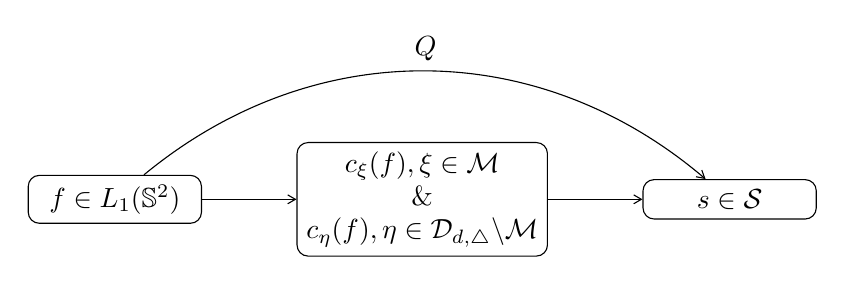
\begin{tikzpicture}[
node distance = 12mm and 12mm, box/.style = {draw, rounded corners, minimum width=22mm, minimum height=5mm, align=center},
> = {Straight Barb[angle=60:2pt 3]},bend angle = 15, auto = left]
\node (n1)  [box]{$f\in L_1(\mathbb S^2)$};
\node (n2)  [box, right=of n1]{$c_\xi(f), \xi\in \mathcal M$\\ \& \\ $c_\eta(f), \eta\in \mathcal D_{d,\triangle}\backslash \mathcal M$};
\node (n4)  [box, right=of n2] {$s \in\mathcal S$};
\draw[->] (n1) to [""] (n2);\draw[->] (n2) to [""] (n4);
\draw[->] (n1) to [bend right=-40, "$Q$"] (n4);
\end{tikzpicture}

\end{document}